\documentclass[a4paper,12pt]{article}
\usepackage{amsmath}
\usepackage{graphicx}
\usepackage[colorlinks=true, allcolors=blue]{hyperref}
\usepackage[utf8]{inputenc}
\usepackage[T1]{fontenc}
\usepackage[english, english]{babel}
\usepackage{color}
\usepackage{fancyhdr}
\usepackage{listings}
\usepackage{array}
\usepackage{caption}
\usepackage{array}
\usepackage[letterpaper,top=2cm,bottom=2cm,left=3cm,right=3cm,marginparwidth=1.75cm]{geometry}
\usepackage{booktabs}
\usepackage{longtable}
\usepackage{float}
\usepackage{minted}
\usepackage{pdflscape}
\usepackage{svg}

\setlength{\parindent}{0pt}
\pagestyle{fancy}
\fancyhf{} % Clear all header and footer fields
\lfoot{Page \thepage} % Left-aligned footer

\pagenumbering{arabic}

\geometry{
  a4paper,
  left=2cm,
  right=2cm,
  top=2cm,
  bottom=2cm
}

\title{PR1 Report}

\begin{document}

\begin{titlepage}

\hspace{-0.75cm}\begin{minipage}{0.4\textwidth}
           \centering 
          
\includegraphics[width=9cm]{logo_IPP.png}
    \end{minipage}
   % \hspace{%cm}
    \begin{minipage}{1\textwidth}
          \centering 
          
\includegraphics[width=4cm,height=5cm]{logo_telecom.png}
    \end{minipage}
    \hspace{0.5cm}

\vspace{2cm}

\begin{center}
        \underline{\textbf{\large\Huge{Télécom paris}}} \\
        \vspace{0.5cm}
    \end{center}
    \vspace{2cm}

    \begin{center}
        \textbf{\large\Huge{Execution Support}}\\
        \vspace{0.5cm}
    \end{center}

    \vspace{1cm}

    \hrule % Ajout d'une ligne horizontale

 

    \begin{center}
    \Large{\textbf{\Huge{{PR1}}}}
    \end{center} 
    
    \hrule % Ajout d'une ligne horizontale
    
    \vspace{1cm}
\begin{center}
   \noindent\large\textbf{Developed by:}\\ 
    \normalsize
     \large {Souhail Ait Fora} \\
    {Said Agouzal} \\
    {Hichem Chtourou} \\  
    \vspace{0.5cm}
    \end{center} 



    
\centering  Academic year: 2024/2025

\end{titlepage}


\newpage
\thispagestyle{empty} 
\tableofcontents

\newpage
\thispagestyle{empty} 


\newpage
\setcounter{page}{1}

% \documentclass{article}
\date{}
\maketitle

\section{Binary Instructions}
In this section, our aim is to decode, and understand the following set of binary instructions :

\begin{verbatim}
0  : 00050893
4  : 00068513
8  : 04088063
c  : 04058263
10 : 04060063
14 : 04d05063
18 : 00088793
1c : 00269713
20 : 00e888b3
24 : 0007a703
28 : 0005a803
2c : 01070733
30 : 00e62023
34 : 00478793
38 : 00458593
3c : 00460613
40 : ff1792e3
44 : 00008067
48 : fff00513
4c : 00008067
50 : fff00513
54 : 00008067
\end{verbatim}%
\subsection{Instructions Decoding}
The decoding of each instruction is detailed here:
\begin{longtable}{|c|c|c|c|c|}
\hline
\textbf{Address} & \textbf{Hexa} & \textbf{Type} & \textbf{Instruction} & \textbf{Alias} \\ \hline
\texttt{0x00} & \texttt{00050893} & \texttt{I} & \texttt{ADDI x17, x10, 0  }  & \texttt{ADDI a7, a0, 0} \\ \hline
\texttt{0x04} & \texttt{00068513} & \texttt{I} & \texttt{ADDI x10, x13, 0  }  & \texttt{ADDI a0, a3, 0} \\ \hline
\texttt{0x08} & \texttt{04088063} & \texttt{B} & \texttt{BEQ  x17, x0, 64 }  & \texttt{BEQ  a7, zero, 64} \\ \hline
\texttt{0x0c} & \texttt{04058263} & \texttt{B} & \texttt{BEQ  x11, x0, 68 }  & \texttt{BEQ  a1, zero, 68} \\ \hline
\texttt{0x10} & \texttt{04060063} & \texttt{B} & \texttt{BEQ  x12, x0, 64 }  & \texttt{BEQ  a2, zero, 64} \\ \hline
\texttt{0x14} & \texttt{04d05063} & \texttt{B} & \texttt{BGE  x0, x13, 64 }  & \texttt{BGE  zero, a3, 64} \\ \hline
\texttt{0x18} & \texttt{00088793} & \texttt{I} & \texttt{ADDI x15, x17, 0  }  & \texttt{ADDI a5, a7, 0} \\ \hline
\texttt{0x1c} & \texttt{00269713} & \texttt{I} & \texttt{SLLI x14, x13, 2  }  & \texttt{SLLI a4, a3, 2} \\ \hline
\texttt{0x20} & \texttt{00e888b3} & \texttt{R} & \texttt{ADD  x17, x17, x14}  & \texttt{ADD  a7, a7, a4} \\ \hline
\texttt{0x24} & \texttt{0007a703} & \texttt{I} & \texttt{LW   x14, 0(x15)  }  & \texttt{LW   a4, 0(a5)} \\ \hline
\texttt{0x28} & \texttt{0005a803} & \texttt{I} & \texttt{LW   x16, 0(x11)  }  & \texttt{LW   a6, 0(a1)} \\ \hline
\texttt{0x2c} & \texttt{01070733} & \texttt{R} & \texttt{ADD  x14, x14, x16}  & \texttt{ADD  a4, a4, a6} \\ \hline
\texttt{0x30} & \texttt{00e62023} & \texttt{S} & \texttt{SW   x14, 0(x12)  }  & \texttt{SW   a2, 0(a4)} \\ \hline
\texttt{0x34} & \texttt{00478793} & \texttt{I} & \texttt{ADDI x15, x15, 4  }  & \texttt{ADDI a5, a5, 4} \\ \hline
\texttt{0x38} & \texttt{00458593} & \texttt{I} & \texttt{ADDI x11, x11, 4  }  & \texttt{ADDI a1, a1, 4} \\ \hline
\texttt{0x3c} & \texttt{00460613} & \texttt{I} & \texttt{ADDI x12, x12, 4  }  & \texttt{ADDI a2, a2, 4} \\ \hline
\texttt{0x40} & \texttt{ff1792e3} & \texttt{B} & \texttt{BNE  x15, x17, -28}  & \texttt{BNE  a5, a7, -28} \\ \hline
\texttt{0x44} & \texttt{00008067} & \texttt{J} & \texttt{JALR x0, x1, 0  }  & \texttt{JALR zero, ra, 0} \\ \hline
\texttt{0x48} & \texttt{fff00513} & \texttt{I} & \texttt{ADDI x10, x0, -1 }  & \texttt{ADDI a0, zero, -1} \\ \hline
\texttt{0x4c} & \texttt{00008067} & \texttt{J} & \texttt{JALR x0, x1, 0  }  & \texttt{JALR zero, ra, 0} \\ \hline
\texttt{0x50} & \texttt{fff00513} & \texttt{I} & \texttt{ADDI x10, x0, -1 }  & \texttt{ADDI a0, zero, -1} \\ \hline
\texttt{0x54} & \texttt{00008067} & \texttt{J} & \texttt{JALR x0, x1, 0  }  & \texttt{JALR zero, ra, 0} \\ \hline
\caption{Instructions Decoding}
\end{longtable}
\label{tab:instructions-decoding}


Finally, we got the following set of instructions:
\begin{verbatim}
 0: ADDI x17, x10, 0 
 4: ADDI x10, x13, 0
 8: BEQ  x17, x0 , 64
 c: BEQ  x11, x0 , 68
10: BEQ  x12, x0 , 64
14: BGE  x0 , x13, 64
18: ADDI x15, x17, 0
1c: SLLI x14, x13, 2
20: ADD  x17, x17, x14
24: LW   x14, 0(x15)
28: LW   x16, 0(x11)
2c: ADD  x14, x14, x16
30: SW   x14, 0(x12)
34: ADDI x15, x15, 4
38: ADDI x11, x11, 4
3c: ADDI x12, x12, 4
40: BNE  x15, x17, -28
44: JALR x0 , x1 , 0
48: ADDI x10, x0 , -1
4c: JALR x0 , x1 , 0
50: ADDI x10, x0 , -1
54: JALR x0 , x1 , 0
\end{verbatim}
\subsection{Branch Delay Slots}

\begin{figure}[H]
\centering
\begin{minipage}{0.45\textwidth}
    \centering
    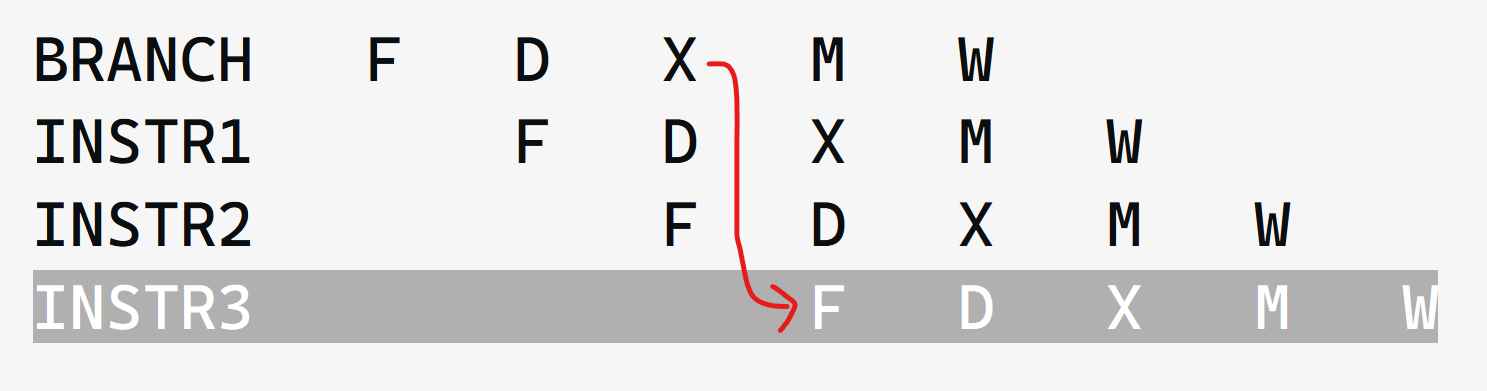
\includegraphics[width=\textwidth]{figure2.png}
    \caption{Illustration of the pipeline.}
    \label{fig:image2}
\end{minipage}%
\hfill % Add space between the images
\begin{minipage}{0.45\textwidth}
    \centering
    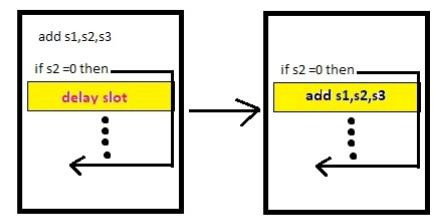
\includegraphics[width=\textwidth]{figure1.jpg}
    \caption{Illustration of delay slots.}
    \label{fig:image1}
\end{minipage}
\end{figure}%
As illustrated in Figure 1, the branch instruction requires two cycles to execute and determine whether the branch is taken or not. During these two cycles, the next two instructions are fetched. If the branch is not taken, these instructions risk being stalled, leading to a waste of two cycles.\\
\\
%
To mitigate this, the branch delay slot optimization is applied by the compiler. This operation involves repositioning two instructions that will always execute, regardless of the branch's outcome, into the delay slots without altering the program's overall behavior. This optimization ensures efficient use of the pipeline and prevents wasted cycles, as shown in Figure 2.\\
\\
%
\textbf{Advantages of Branch Delay Slots :}\\
\\
%
\textbf{Improved Pipelining :} Branch delay slots help to avoid pipeline stalls by allowing the processor to continue executing useful instructions instead of idling while waiting for the branch decision.\\
\\
%
\textbf{Simple to Implement :} For early RISC processors like MIPS, the design of branch delay slots was simple and efficient, and it avoided the need for complex branch prediction mechanisms that were harder to implement at the time.\\
\\
%
\textbf{Disadvantages of Branch Delay Slots :}\\
\\
%
\textbf{Wasted Instruction Cycles :} If the instruction in the delay slot is not useful, the branch delay slot effectively wastes a cycle.\\
\\
%
\textbf{Compiler Responsibility :} The burden is placed on compilers or programmers to fill the branch delay slot with meaningful instructions. This adds complexity to code generation or assembly programming.\\
\\
%
\textbf{Code Readability and Maintainability :} Since the branch delay slot executes the next instruction regardless of the branch, the code flow becomes less predictable and harder to understand.

\subsection{Branches}
In our code, the branch instructions are as the following :\\
\\
%
Address 08 :\\
\texttt{BEQ} instruction jumps to address 48 to execute \texttt{ADDI x10, x0, -1}\\
\\
%
Address 0c :\\
\texttt{BEQ} instruction jump to address 50 to execute \texttt{ADDI x10, x0, -1}\\
\\
%
Address 10 :\\
\texttt{BEQ} instruction jump to address 48 to execute \texttt{ADDI x10, x0, -1}\\
\\
%
Address 14 :\\
\texttt{BGE} instruction jump to address 54 to execute \texttt{JALR x0, x1, 0}\\
\\
%
Address 40 :\\
\texttt{BNE} instruction jump to address 24 to execute \texttt{LW x14, 0(x15)}
\subsection{Signification of the program}
To understand the code, we rewrote it in C language in section 2.\\
\\
%
The function accepts the starting addresses of three arrays of integers and their size as inputs. It then calculates the sum of the corresponding elements from the first two arrays, four bytes at a time, and stores the results in the third array. If any of the provided starting addresses are NULL, the function returns -1 to indicate an error, and if the size is strictly negative, the function returns this value. Otherwise, it performs the calculations as expected and returns the size to indicate a successful execution.
\section{RISC-V tool chain}
\subsection{The C code}
The C translation of our set of instructions is as following :

\inputminted{c}{se201-prog.c}
\subsection{Disassembling the code}
To compile the program we use the following command :\\
\texttt{riscv64-unknown-elf-gcc -g -O0 -mcmodel=medlow -mabi=ilp32 -march=rv32im -Wall -c -o se201-prog.o se201-prog.c}\\\\
%
We disassemble the object file using the command :\\
\texttt{riscv64-unknown-elf-objdump -d se201-prog.o}\\\\
%
We get the following assembler code that we commented for it be more clear :
\begin{verbatim}
00000000 <sum>:
// stack management
   0:	fd010113          	add	sp,sp,-48
   4:	02812623          	sw	s0,44(sp)
   8:	03010413          	add	s0,sp,48
// storing the function arguments in the stack.
   c:	fca42e23          	sw	a0,-36(s0)
  10:	fcb42c23          	sw	a1,-40(s0)
  14:	fcc42a23          	sw	a2,-44(s0)
  18:	fcd42823          	sw	a3,-48(s0)
// uint32_t START1_x17 = x10 + 0;
  1c:	fdc42783          	lw	a5,-36(s0)
  20:	fef42423          	sw	a5,-24(s0)
// x10 = NINTS_x13 + 0;
  24:	fd042783          	lw	a5,-48(s0)
  28:	fcf42e23          	sw	a5,-36(s0)
// if (START1_x17 == 0) goto L48;
  2c:	fe842783          	lw	a5,-24(s0)
  30:	0a078863          	beqz	a5,e0 <.L13>
// if (START2_x11 == 0) goto L50;
  34:	fd842783          	lw	a5,-40(s0)
  38:	0c078263          	beqz	a5,fc <.L14>
// if (STARTR_x12 == 0) goto L48;
  3c:	fd442783          	lw	a5,-44(s0)
  40:	0a078463          	beqz	a5,e8 <.L15>
// if (0 >= x13) goto L54;
  44:	fd042783          	lw	a5,-48(s0)
  48:	0cf05263          	blez	a5,10c <.L16>
// uint32_t START1_x15 = START1_x17;
  4c:	fe842783          	lw	a5,-24(s0)
  50:	fef42623          	sw	a5,-20(s0)
// uint32_t NBYTE_x14 = NINTS_x13 << 2;
  54:	fd042783          	lw	a5,-48(s0)
  58:	00279793          	sll	a5,a5,0x2
  5c:	fef42223          	sw	a5,-28(s0)
// END1_x17 = START1_x17 + NBYTE_x14;
  60:	fe842703          	lw	a4,-24(s0)
  64:	fe442783          	lw	a5,-28(s0)
  68:	00f707b3          	add	a5,a4,a5
  6c:	fef42423          	sw	a5,-24(s0)

00000070 <.L9>:
  // x14 = *(uint32_t *)(START1_x15);
  70:	fec42783          	lw	a5,-20(s0)
  74:	0007a783          	lw	a5,0(a5)
  78:	fef42223          	sw	a5,-28(s0)
// uint32_t x16 = *(uint32_t *)(START2_x11);
  7c:	fd842783          	lw	a5,-40(s0)
  80:	0007a783          	lw	a5,0(a5)
  84:	fef42023          	sw	a5,-32(s0) x16
// x14 = x14 + x16;
  88:	fe442703          	lw	a4,-28(s0)
  8c:	fe042783          	lw	a5,-32(s0)
  90:	00f707b3          	add	a5,a4,a5
  94:	fef42223          	sw	a5,-28(s0)
// *(uint32_t *)(x12) = x14;
  98:	fd442783          	lw	a5,-44(s0)
  9c:	fe442703          	lw	a4,-28(s0)
  a0:	00e7a023          	sw	a4,0(a5)
// START1_x15 = START1_x15 + 4;
  a4:	fec42783          	lw	a5,-20(s0)
  a8:	00478793          	add	a5,a5,4
  ac:	fef42623          	sw	a5,-20(s0)
// START2_x11 = START2_x11 + 4;
  b0:	fd842783          	lw	a5,-40(s0)
  b4:	00478793          	add	a5,a5,4
  b8:	fcf42c23          	sw	a5,-40(s0)
// STARTR_x12 = STARTR_x12 + 4;
  bc:	fd442783          	lw	a5,-44(s0)
  c0:	00478793          	add	a5,a5,4
  c4:	fcf42a23          	sw	a5,-44(s0)
// if (START1_x15 != END1_x17) goto L44;
  c8:	fec42703          	lw	a4,-20(s0)
  cc:	fe842783          	lw	a5,-24(s0)
  d0:	00f70463          	beq	a4,a5,d8 <.L10>
  d4:	f9dff06f          	j	70 <.L9>

// defining the return value as x10 and go to the return bloc (L11)
000000d8 <.L10>:
  d8:	fdc42783          	lw	a5,-36(s0)
  dc:	0380006f          	j	114 <.L11>

000000e0 <.L13>:
  e0:	00000013          	nop
  e4:	0080006f          	j	ec <.L3>

000000e8 <.L15>:
  e8:	00000013          	nop

// defining the return value as -1 = x10 and go to the return bloc (L10)
000000ec <.L3>:
  ec:	fff00793          	li	a5,-1
  f0:	fcf42e23          	sw	a5,-36(s0)
  f4:	fdc42783          	lw	a5,-36(s0)
  f8:	01c0006f          	j	114 <.L11>

000000fc <.L14>:
  fc:	00000013          	nop

//same as L3
00000100 <.L5>:
 100:	fff00793          	li	a5,-1
 104:	fcf42e23          	sw	a5,-36(s0)
 108:	0080006f          	j	110 <.L8>

0000010c <.L16>:
 10c:	00000013          	nop

00000110 <.L8>:
 110:	fdc42783          	lw	a5,-36(s0)

// stack management and returning 
00000114 <.L11>:
 114:	00078513          	mv	a0,a5
 118:	02c12403          	lw	s0,44(sp)
 11c:	03010113          	add	sp,sp,48
 120:	00008067          	ret
\end{verbatim}
%
This code was generated without applying any compiler optimizations. As a result, it exhibits several characteristics that contribute to increased complexity and size compared to the initial set of instructions:\\
\\
%
\textbf{Stack management and calling conventions :}\\
The compiler adheres strictly to calling conventions, ensuring that the code is compatible with general use cases.\\
\\
%
\textbf{The stack excessive usage :}\\
Without optimizations, the compiler fails to make efficient use of available registers. Instead, it relies heavily on memory regions in the stack to store local variables. Consequently, it frequently employs load and store instructions whenever these variables are accessed, leading to inefficiencies.\\
\\
%
\textbf{The excessive creation of labels :}\\
The absence of optimizations causes the compiler to generate a distinct label for every conditional instruction, further increasing the complexity of the code.

\subsection{Adding O3 optimization}
When activating the O3 optimization, we get the following code :
\begin{verbatim}
00000000 <sum>:
// if (START1_x17 == 0) goto L48;
   0:	04050663          	beqz	a0,4c <.L2>
// if (START2_x11 == 0) goto L50;
   4:	04058463          	beqz	a1,4c <.L2>
// if (STARTR_x12 == 0) goto L48;
   8:	04060263          	beqz	a2,4c <.L2>
// if (0 >= x13) goto L54;
   c:	02d05c63          	blez	a3,44 <.L5>

00000010 <.LVL1>:
// uint32_t NBYTE_x14 = NINTS_x13 << 2;
  10:	00269313          	sll	t1,a3,0x2

00000014 <.LVL2>:
// uint32_t START1_x15 = START1_x17;
  14:	00050793          	mv	a5,a0
// END1_x17 = START1_x17 + NBYTE_x14;
  18:	00a30333          	add	t1,t1,a0

0000001c <.LVL3>:
// a2 becomes the offset between the starting adresses of the first input 
array and the result array
  1c:	40a60633          	sub	a2,a2,a0

00000020 <.LVL4>:
// a1 becomes the difference between the starting adresses of the two input 
arrays
  20:	40a585b3          	sub	a1,a1,a0

00000024 <.L4>:
// a4(address of the second input array) is calculated using a5(address of 
the first input array) and the offset
  24:	00f58733          	add	a4,a1,a5
// x14 = *(uint32_t *)(START1_x15);
  28:	0007a883          	lw	a7,0(a5)

0000002c <.LVL6>:
// uint32_t x16 = *(uint32_t *)(START2_x11);
  2c:	00072703          	lw	a4,0(a4)
// a6(address of the result array) is calculated using a5(address of the 
first input array) and the offset
  30:	00f60833          	add	a6,a2,a5
// start* = start* + 4;
  34:	00478793          	add	a5,a5,4

00000038 <.LVL7>:
// x14 = x14 + x16;
  38:	01170733          	add	a4,a4,a7
// *(uint32_t *)(x12) = x14;
  3c:	00e82023          	sw	a4,0(a6)

00000040 <.LVL8>:
// if (START1_x15 != END1_x17) goto L24;
  40:	fef312e3          	bne	t1,a5,24 <.L4>

00000044 <.L5>:
// return x10;
  44:	00068513          	mv	a0,a3
  48:	00008067          	ret

0000004c <.L2>:
//return -1
  4c:	fff00513          	li	a0,-1

00000050 <.LDL1>:
  50:	00008067          	ret
\end{verbatim}%
In contrast to the optimization-less code, this version is shorter and more closely resembles the initial instruction set. The primary difference lies in the use of offsets, which eliminates the need to repeatedly increment each array address by 4.\\
%
This assembly program does not adhere to any calling conventions, as it fully utilizes the available registers and avoids using the stack to store local variables. Additionally, it generates only a single label to manage branch instructions, resulting in a more efficient implementation.
\section{RISC-V Architecture}
\subsection{Program Flow}
The following table presents the execution of the program of Section 1, with the value of the different registers and explanation of each instruction.\\
\\
%
The program starts with the following initial processor state:
\begin{itemize}
    \item The registers a0, a1, and a2 all have the value 0x200.
    \item The a3 register has the value 0x2.
    \item All other registers have the value zero (0x0).
    \item The memory contents in the address range 0x200 through 0x210 are given as follows:
\end{itemize}
\begin{verbatim}
                                Address Value
                                0x200   0x61
                                0x204   0x20
                                0x208   0x62
                                0x20C   0x0
                                0x210   0x0
\end{verbatim}
\begin{itemize}
    \item All other memory cells have a value of zero (0x0).
\end{itemize}
\newpage
\begin{landscape}


\begin{longtable}{|c c c c c c c c c c p{8cm}|}
\hline
\texttt{PC}    & \textbf{INSTRUCTION}     & \texttt{a0}    & \texttt{a1}    & \texttt{a2}    & \texttt{a3}  & \texttt{a4}   & \texttt{a5}    & \texttt{a6}   & \texttt{a7}    & \textbf{EXPLANATION}\\
\hline
\texttt{0x0}  & \texttt{ADDI a7, a0, 0}  & \texttt{0x200} & \texttt{0x200} & \texttt{0x200} & \texttt{0x2} & \texttt{0x0}  & \texttt{0x0}   & \texttt{0x0}  & \texttt{0x200} & Copy value of a0 into a7\\
\hline
\texttt{0x4}  & \texttt{ADDI a0, a3, 0}  & \texttt{0x2}   & \texttt{0x200} & \texttt{0x200} & \texttt{0x2} & \texttt{0x0}  & \texttt{0x0}   & \texttt{0x0}  & \texttt{0x200} & Copy value of a3 into a0\\
\hline
\texttt{0x8}  & \texttt{BEQ a7, x0, 64}  & \texttt{0x2}   & \texttt{0x200} & \texttt{0x200} & \texttt{0x2} & \texttt{0x0}  & \texttt{0x0}   & \texttt{0x0}  & \texttt{0x200} & PC = PC + 64 = 0x48 if a7 = 0. This branch is not taken.\\
\hline
\texttt{0xc}  & \texttt{BEQ a1, x0, 68}  & \texttt{0x2}   & \texttt{0x200} & \texttt{0x200} & \texttt{0x2} & \texttt{0x0}  & \texttt{0x0}   & \texttt{0x0}  & \texttt{0x200} & PC = PC + 68 = 0x50 if a1 = 0. This branch is not taken.\\
\hline
\texttt{0x10} & \texttt{BEQ a2, x0, 64}  & \texttt{0x2}   & \texttt{0x200} & \texttt{0x200} & \texttt{0x2} & \texttt{0x0}  & \texttt{0x0}   & \texttt{0x0}  & \texttt{0x200} & PC = PC + 64 = 0x50 if a2 = 0. This branch is not taken.\\
\hline
\texttt{0x14} & \texttt{BGE x0, a3, 64}  & \texttt{0x2}   & \texttt{0x200} & \texttt{0x200} & \texttt{0x2} & \texttt{0x0}  & \texttt{0x0}   & \texttt{0x0}  & \texttt{0x200} & PC = PC + 64 = 0x54 if a3 < 0. This branch is not taken.\\
\hline
\texttt{0x18} & \texttt{ADDI a5, a7, 0}  & \texttt{0x2}   & \texttt{0x200} & \texttt{0x200} & \texttt{0x2} & \texttt{0x0}  & \texttt{0x200} & \texttt{0x0}  & \texttt{0x200} & Copy value of a7 into a5\\
\hline
\texttt{0x1c} & \texttt{SLLI a4, a3, 2}  & \texttt{0x2}   & \texttt{0x200} & \texttt{0x200} & \texttt{0x2} & \texttt{0x8}  & \texttt{0x200} & \texttt{0x0}  & \texttt{0x200} & Multiply value of a3 by 4 and copy it into a4\\
\hline
\texttt{0x20} & \texttt{ADD a7, a7, a4}  & \texttt{0x2}   & \texttt{0x200} & \texttt{0x200} & \texttt{0x2} & \texttt{0x8}  & \texttt{0x200} & \texttt{0x0}  & \texttt{0x208} & Copy sum of a7 and a4 into a7. This instruction needs forwarding of the value of a4 from the previous instruction.\\
\hline
\texttt{0x24} & \texttt{LW a4, 0(a5)}    & \texttt{0x2}   & \texttt{0x200} & \texttt{0x200} & \texttt{0x2} & \texttt{0x61} & \texttt{0x200} & \texttt{0x0}  & \texttt{0x208} & Copy the content at address 0X200 into a4\\
\hline
\texttt{0x28} & \texttt{LW a6, 0(a1)}    & \texttt{0x2}   & \texttt{0x200} & \texttt{0x200} & \texttt{0x2} & \texttt{0x61} & \texttt{0x200} & \texttt{0x61} & \texttt{0x208} & Copy the content at address 0X200 into a6\\
\hline
\texttt{0x2c} & \texttt{ADD a4, a4, a6}  & \texttt{0x2}   & \texttt{0x200} & \texttt{0x200} & \texttt{0x2} & \texttt{0xc2} & \texttt{0x200} & \texttt{0x61} & \texttt{0x208} & Copy the sum of a4 and a6 into a4. This instruction needs to stall in the ID stage waiting for a6 to be written from the previous load instruction and to get the value of a6 by forwarding its value from the previous instruction's WB stage\\
\hline
\texttt{0x30} & \texttt{SW a4, 0(a2)}    & \texttt{0x2}   & \texttt{0x200} & \texttt{0x200} & \texttt{0x2} & \texttt{0xc2} & \texttt{0x200} & \texttt{0x61} & \texttt{0x208} & Store a4 at address 0x200, now this address holds its previous value multiplied by 2. This instruction needs the value of a4, therefore needs forwarding it from the previous instruction's MEM stage\\
\hline
\texttt{0x34} & \texttt{ADDI a5, a5, 4}  & \texttt{0x2}   &\texttt{0x200} & \texttt{0x200} & \texttt{0x2} & \texttt{0xc2} & \texttt{0x204} & \texttt{0x61} & \texttt{0x208} & Copy the value of a5 + 4 into a5\\
\hline
\texttt{0x38} & \texttt{ADDI a1, a1, 4}  & \texttt{0x2}   & \texttt{0x204} & \texttt{0x200} & \texttt{0x2} & \texttt{0xc2} & \texttt{0x204} & \texttt{0x61} & \texttt{0x208} & Copy the value of a1 + 4 into a1\\
\hline
\texttt{0x3c} & \texttt{ADDI a2, a2, 4}  & \texttt{0x2}   & \texttt{0x204} & \texttt{0x204} & \texttt{0x2} & \texttt{0xc2} & \texttt{0x204} & \texttt{0x61} & \texttt{0x208} & Copy the value of a2 + 4 into a2\\
\hline
\texttt{0x40} & \texttt{BNE a5, a7, -28} & \texttt{0x2}   & \texttt{0x204} & \texttt{0x204} & \texttt{0x2} & \texttt{0xc2} & \texttt{0x204} & \texttt{0x61} & \texttt{0x208} & PC = PC - 28 = 0x24 if a5 != a7. This branch is taken, so we have to flush the next two instructions at ID and IF stages respectively. \\
\hline
\texttt{0x24} & \texttt{LW a4, 0(a5)}    & \texttt{0x2}   & \texttt{0x204} & \texttt{0x204} & \texttt{0x2} & \texttt{0x20} & \texttt{0x204} & \texttt{0x61} & \texttt{0x208} & Copy the content at address 0x204 into a4\\
\hline
\texttt{0x28} & \texttt{LW a6, 0(a1)}    & \texttt{0x2}   & \texttt{0x204} & \texttt{0x204} & \texttt{0x2} & \texttt{0x20} & \texttt{0x204} & \texttt{0x20} & \texttt{0x208} & Copy the content at address 0x204 into  a6\\
\hline
\texttt{0x2c} & \texttt{ADD a4, a4, a6}  & \texttt{0x2}   & \texttt{0x204} & \texttt{0x204} & \texttt{0x2} & \texttt{0x40} & \texttt{0x204} & \texttt{0x20} & \texttt{0x208} & Copy the sum of a4 and a6 into a4. This instruction needs to stall in the ID stage waiting for a6 to be written from the previous load instruction and to get the value of a6 by forwarding its value from the previous instruction's WB stage\\
\hline
\texttt{0x30} & \texttt{SW a4, 0(a2)}    & \texttt{0x2}   & \texttt{0x204} & \texttt{0x204} & \texttt{0x2} & \texttt{0x40} & \texttt{0x204} & \texttt{0x20} & \texttt{0x208} & Store value of a4 in the memory case having the address contained in a2, now address 0x204 holds the previous value it held multiplied by 2. This instruction will need the value of a4 to store it in a memory case therefore it will need forwarding of a4 value from the previous instruction's MEM stage\\
\hline
\texttt{0x34} & \texttt{ADDI a5, a5, 4}  & \texttt{0x2}   & \texttt{0x204} & \texttt{0x204} & \texttt{0x2} & \texttt{0x40} & \texttt{0x208} & \texttt{0x20} & \texttt{0x208} & Copy the value of a5 + 4 into a5\\
\hline
\texttt{0x38} & \texttt{ADDI a1, a1, 4}  & \texttt{0x2}   & \texttt{0x208} & \texttt{0x204} & \texttt{0x2} & \texttt{0x40} & \texttt{0x208} & \texttt{0x20} & \texttt{0x208} & Copy the value of a1 + 4 into a1\\
\hline
\texttt{0x3c} & \texttt{ADDI a2, a2, 4}  & \texttt{0x2}   & \texttt{0x208} & \texttt{0x208} & \texttt{0x2} & \texttt{0x40} & \texttt{0x208} & \texttt{0x20} & \texttt{0x208} & Copy the value of a2 + 4 into a2\\
\hline
\texttt{0x40} & \texttt{BNE a5, a7, -28} & \texttt{0x2}   & \texttt{0x208} & \texttt{0x208} & \texttt{0x2} & \texttt{0x40} & \texttt{0x208} & \texttt{0x20} & \texttt{0x208} & PC = PC - 28 = 0x24 if a5 != a7. This branch is not taken because a5 = a7 = 0x208\\
\hline
\texttt{0x44} & \texttt{JALR x0, x1, 0}  & \texttt{0x2}   & \texttt{0x204} & \texttt{0x200} & \texttt{0x2} & \texttt{0xc2} & \texttt{0x204} & \texttt{0x61} & \texttt{0x208} & End of function. We return a0  =  0x2\\
\hline

\caption{Instruction Execution Table}
\end{longtable}

\label{tab:instruction_execution}


\end{landscape}
\newpage

\subsection{Pipeline Diagram}
The following figure is the pipeline diagram, which represents the propagation of the different instructions inside the processor.
\begin{figure}[H]
    \centering
    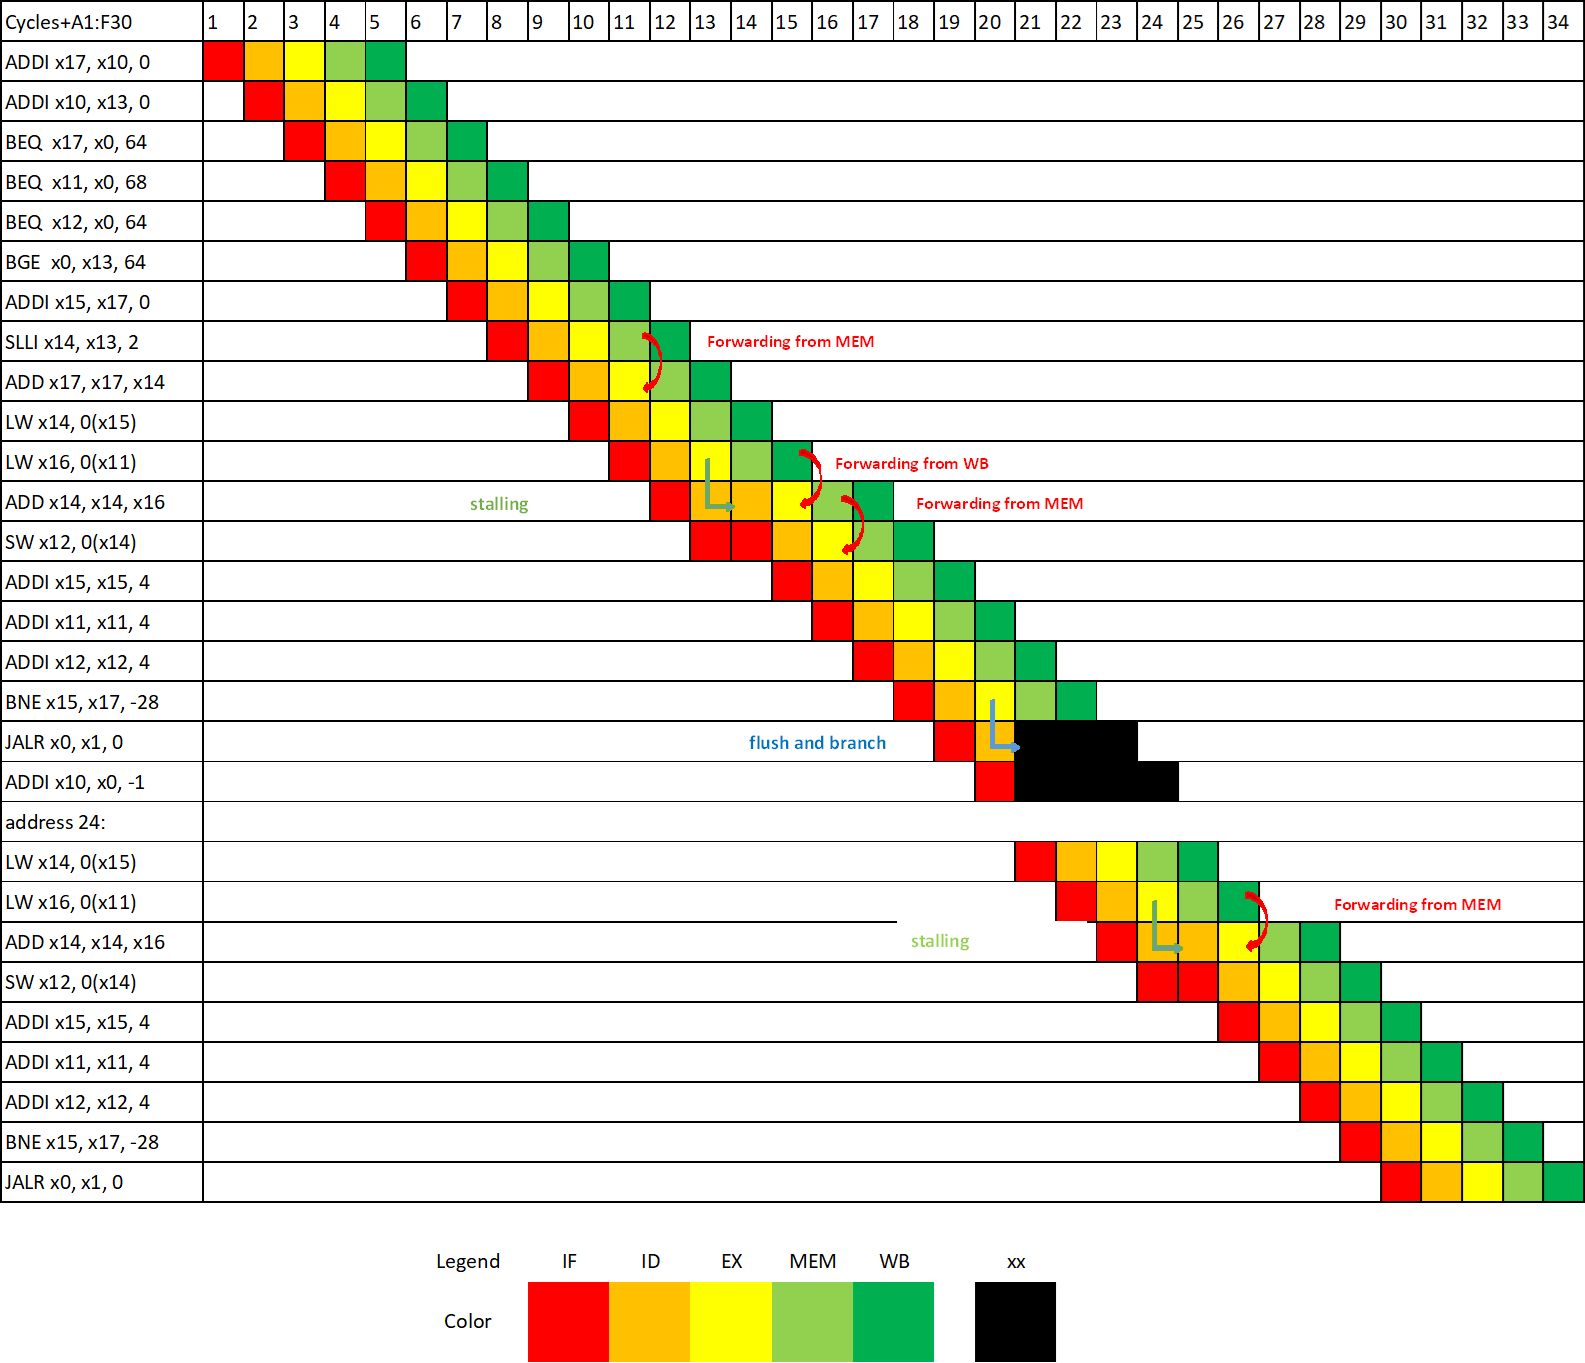
\includegraphics[width=1\linewidth]{pipeline.png}
    \caption{Pipeline diagram}
    \label{fig:pipeline diagram}
\end{figure}
\section{Processor Design}
\subsection{Instruction Set Architecture}
For our instruction set, we chose an implementation with the following characteristics :\\

\textbf{Registers usage :}\\

Our implementation contains 16 registers from r0 to r15. r1 is the return address register, as it store the address from which a function is called. The registers from r10 to r13 are the function arguments and r10 is also the return value of this function. Additionally, the registers r14 and r15 are the stack pointer and the program counter respectively. Finally, r0 is a special register that can receive the return value of some 2 registers instructions. \\
Before calling a function, the arguments should be passed in the r10 to r13 registers, and the call instruction should normally store the return address in r1. To return from a function call, the return value should be stored in r10, and a jump instruction to r1 should be executed.\\

\textbf{Instructions :}\\\\
%
Table 4 presents our instruction set. After dividing our instructions into different types, we get the following decoding table :
\begin{table}[H]
\centering\begin{tabular}{lclclclcccc}
                              & \multicolumn{2}{l}{\texttt{15\hspace{1cm}12}} & \multicolumn{2}{l}{\texttt{11\hspace{1cm}8}}                                     & \multicolumn{2}{l}{\texttt{7\hspace{1cm}4}} & \texttt{3}                      & \texttt{2}                               & \texttt{1}                               & \texttt{0}                      \\ \hline
\multicolumn{1}{|l|}{O-Type}  & \multicolumn{2}{c|}{rd}             & \multicolumn{2}{c|}{rs1}              & \multicolumn{2}{c|}{func3}            & \multicolumn{4}{c|}{1001}                                                                                           \\ \hline
\multicolumn{1}{|l|}{D-Type}  & \multicolumn{2}{c|}{func2}          & \multicolumn{2}{c|}{rs1}              & \multicolumn{2}{c|}{rs2}             & \multicolumn{4}{c|}{0111}                                                                                           \\ \hline
\multicolumn{1}{|l|}{T-Type}  & \multicolumn{2}{c|}{rd}             & \multicolumn{2}{c|}{rs1}              & \multicolumn{2}{c|}{rs2}             & \multicolumn{4}{c|}{func1}                                                                                          \\ \hline
\multicolumn{1}{|l|}{B-Type}  & \multicolumn{2}{c|}{imm{[}9:6{]}}   & \multicolumn{2}{c|}{rs1}              & \multicolumn{4}{c|}{imm{[}5:0{]}}                                                               & \multicolumn{2}{c|}{00}                                  \\ \hline
\multicolumn{1}{|l|}{J-Type}  & \multicolumn{2}{c|}{0000}           & \multicolumn{2}{c|}{rs1}              & \multicolumn{2}{c|}{0000}            & \multicolumn{4}{c|}{1001}                                                                                           \\ \hline
\multicolumn{1}{|l|}{L-Type}  & \multicolumn{2}{c|}{rd}             & \multicolumn{2}{c|}{rs1}              & \multicolumn{2}{c|}{imm{[}4:1{]}}    & \multicolumn{2}{c|}{00}                                  & \multicolumn{1}{l|}{imm{[}0{]}} & \multicolumn{1}{c|}{1} \\ \hline
\multicolumn{1}{|l|}{S-Type}  & \multicolumn{2}{c|}{imm{[}4:1{]}}   & \multicolumn{2}{c|}{rs1}              & \multicolumn{2}{c|}{rs2}             & \multicolumn{1}{c|}{0} & \multicolumn{1}{c|}{imm{[}0{]}} & \multicolumn{2}{c|}{10}                                  \\ \hline
\multicolumn{1}{|l|}{CL-Type} & \multicolumn{6}{c|}{imm{[}11:0{]}}                                                                                 & \multicolumn{4}{c|}{0101}                                                                                           \\ \hline
\multicolumn{1}{|l|}{CP-Type} & \multicolumn{2}{c|}{rd}             & \multicolumn{4}{c|}{imm{[}7:0{]}}                                            & \multicolumn{4}{c|}{1111}                                                                                           \\ \hline
\multicolumn{1}{|l|}{I-Type}  & \multicolumn{2}{c|}{func2}          & \multicolumn{2}{c|}{rs1}              & \multicolumn{2}{c|}{imm{[}3:0{]}}             & \multicolumn{4}{c|}{0111}                                                                                           \\ \hline
\end{tabular}
\caption{Decoding table}
\end{table}
\label{tab:decoding_table}
The nop operation is \texttt{addi r0, 0} so it's binary form would be \texttt{0100 0000 0000 0111}.


\begin{landscape}
\begin{table}[]
\begin{tabular}{|l|l|l|l|l|}
\hline
\textbf{Instruction}      & \textbf{Type} & \textbf{Role}                                    & \textbf{Binary form}                                           & \textbf{Sign extended} \\ \hline
\texttt{bne rs1, imm}     & \textbf{B}    & \texttt{pc = pc + imm * 2 if rs1 != 0}           & \texttt{imm{[}9:6{]} rs1{[}3:0{]} imm{[}5:0{]} 00}             & yes           \\ \hline
\texttt{lw rd, imm(rs1)}  & \textbf{L}    & \texttt{rd = mem{[}rs1 + imm{]}}                 & \texttt{rd{[}3:0{]} rs1{[}3:0{]} imm{[}4:1{]} 00 imm{[}0{]} 1} & yes           \\ \hline
\texttt{sw rs2, imm(rs1)} & \textbf{S}    & \texttt{mem{[}rs1 + imm{]} = rs2}                & \texttt{imm{[}4:1{]} rs1{[}3:0{]} rs2{[}3:0{]} 0 imm{[}0{]} 10}& yes           \\ \hline
\texttt{call imm}         & \textbf{CL}   & \texttt{r1 = pc; pc = imm}                       & \texttt{imm{[}11:0{]} 0101}                                    & no            \\ \hline
\texttt{jal rs1}          & \textbf{J}    & \texttt{pc = rs1}                                & \texttt{0000 rs1{[}3:0{]} 0000 1001}                           & -             \\ \hline
\texttt{not rd, rs1}      & \textbf{O}    & \texttt{rd = $\sim$rs1}                          & \texttt{rd{[}3:0{]} rs1{[}3:0{]} 0001 1001}                    & -             \\ \hline 
 \texttt{mv rd, rs1}& \textbf{O}& \texttt{rd = rs1}& \texttt{rd{[}3:0{]} rs1{[}3:0{]} 0010 1001}&-\\\hline
\texttt{add rd, rs1, rs2} & \textbf{T}    & \texttt{rd = rs1 + rs2}                          & \texttt{rd{[}3:0{]} rs1{[}3:0{]} rs2{[}3:0{]} 1010}            & -             \\ \hline
\texttt{sub rd, rs1, rs2} & \textbf{T}    & \texttt{rd = rs1 - rs2}                          & \texttt{rd{[}3:0{]} rs1{[}3:0{]} rs2{[}3:0{]} 1011}            & -             \\ \hline
\texttt{cp rd, imm}       & \textbf{CP}   & \texttt{rd = imm}                                & \texttt{rd{[}3:0{]} imm{[}7:0{]} 1111}                         & no            \\ \hline
\texttt{sll rd, rs1, rs2} & \textbf{T}    & \texttt{rd = rs1 \textless{}\textless rs2}       & \texttt{rd{[}3:0{]} rs1{[}3:0{]} rs2{[}3:0{]} 1101}            & -             \\ \hline
\texttt{srl rd, rs1, rs2} & \textbf{T}    & \texttt{rd = rs1 \textgreater{}\textgreater rs2} & \texttt{rd{[}3:0{]} rs1{[}3:0{]} rs2{[}3:0{]} 1110}            & -             \\ \hline
\texttt{get rs1, rs2}     & \textbf{D}    & \texttt{r0 = (rs1 \textgreater{}= rs2) ? 1 : 0}  & \texttt{0000 rs1{[}3:0{]} rs2{[}3:0{]} 0111}                   & -             \\ \hline
\texttt{lt rs1, rs2}      & \textbf{D}    & \texttt{r0 = (rs1 \textless rs2) ? 1 : 0}        & \texttt{0001 rs1{[}3:0{]} rs2{[}3:0{]} 0111}                   & -             \\ \hline
\texttt{slli rs1, imm}   & \textbf{I}    & \texttt{r0 = rs1 \textless{}\textless imm}       & \texttt{1000 rs1{[}3:0{]} imm{[}3:0{]} 0111}                   & no            \\ \hline
\texttt{addi rs1, imm}    & \textbf{I}    & \texttt{r0 = rs1 + imm}& \texttt{0100 rs1{[}3:0{]} imm{[}3:0{]} 0111}                   & yes\\ \hline
\texttt{nand rs1, rs2}    & \textbf{D}    & \texttt{r0 = $\sim$(rs1 \& rs2)}                 & \texttt{0010 rs1{[}3:0{]} rs2{[}3:0{]} 0111}                   & -             \\ \hline
\texttt{or rs1, rs2}      & \textbf{D}    & \texttt{r0 = rs1 | rs2}                          & \texttt{0010 rs1{[}3:0{]} rs2{[}3:0{]} 0111}                   & -             \\ \hline
\texttt{xor rs1, rs2}     & \textbf{D}    & \texttt{r0 = rs1 \textasciicircum rs2}           & \texttt{0011 rs1{[}3:0{]} rs2{[}3:0{]} 0111}                   & -             \\ \hline
\end{tabular}
\caption{Instruction set}
\end{table}
\label{tab:instruction_set}
\end{landscape}
\textbf{Sum function :}\\

The following code is an implementation of the function that computes the sum of two integers, and another function that calls the first one with arguments 63408 and 134.
\begin{verbatim}
0x00 main :
0x0 : cp r10, #0x80
0x2 : cp r11, #0xff
0x4 : slli r11, #8
0x6 : add r10, r10, r0
0x8 : call 0x20
0xa : cp r11, #134 (branch delay slot)
    
0xc : cp x0, #1
0x0e end :
0xe : bne x0, #0x1c
0x10 : nop (branch delay slot)
    
0x12 func-sum :
0x12 : jal r1
0x14 : add r10, r10, r11 (branch delay slot)
\end{verbatim}
\textbf{Initial Function Re-implementation :}\\

We also used our instruction set to re implement the program from section 1. The arguments are assumed to be in r10, r11, r12, r13. Where r10, r11 and r12 
are the starting addresses of arrays 1, 2 and the result array respectively,and 
r13 is the size of the arrays. Also, we assume that this function was already called, so r1 has a return address.
\begin{verbatim}

0x0 sum :
@stack management
0x00 : cp r0, #16
0x02 : sub r14, r14, r0

0x04 : sw r2, 12(r14) @saving r2, a callee saved register
0x08 : mv r2, r10
0x06 : bne r2, #4
0x08 : cp r0, #0x58 (branch delay slot)
0x0c : jal r0
0x0e : nop (branch delay slot)
0x10 : bne r11, #4
0x12 : mv r10, r13 (branch delay slot)
0x14 : jal r0
0x16 : nop (branch delay slot)
0x18 : bne r12, #4
0x1a : nop (branch delay slot)
0x1c : jal r0
0x1e : nop (branch delay slot)
0x20 : cp r0, #0
0x22 : lt r13, r0
0x24 : bne r0, #29
0x26 : nop (branch delay slot)

0x28 : sw r3, 8(r14) @saving r3, a callee saved register
0x2a : mv r3, r2
0x2c : sw r4, 4(r14) @saving r4, a callee saved register
0x2e : slli r4, r13, 2
0x30 : add r2, r2, r4
0x32 : lw r4, 0(r3)
0x34 : sw r5, 0(r14) @saving r5, a callee saved register
0x36 : lw r5, 0(r11)
0x38 : add r4, r4, r5
0x3a : sw r4, 0(r12)
0x3c : cp r0, #4
0x3e : add r3, r3, r0
0x40 : add r11, r11, r0
0x42 : add r12, r12, r0
0x44 : sub r0, r2, r3
0x46 : bne r0, #-20
0x48 : nop (branch delay slot)
0x4a : lw r2, 12(r14)
0x4c : lw r3, 8(r14)
0x4e : lw r4, 4(r14)
0x50 : lw r5, 0(r14)
0x52 : addi r14, 16
0x54 : jal r1
0x56 : mv r14, r0 (branch delay slot)

0x58 : cp r0, #0
0x5a : addi r0, #-1
0x5c : mv r10, r0
0x5e : lw r2, 12(r14)
0x60 : addi r14, 16
0x62 : jal r1
0x64 : mv r14, r0 (branch delay slot)
\end{verbatim}


\subsection{Pipelining}
In this section, we propose a scheme for our processor that handles the different instructions in our instruction set.\\

\begin{figure}
    \centering
    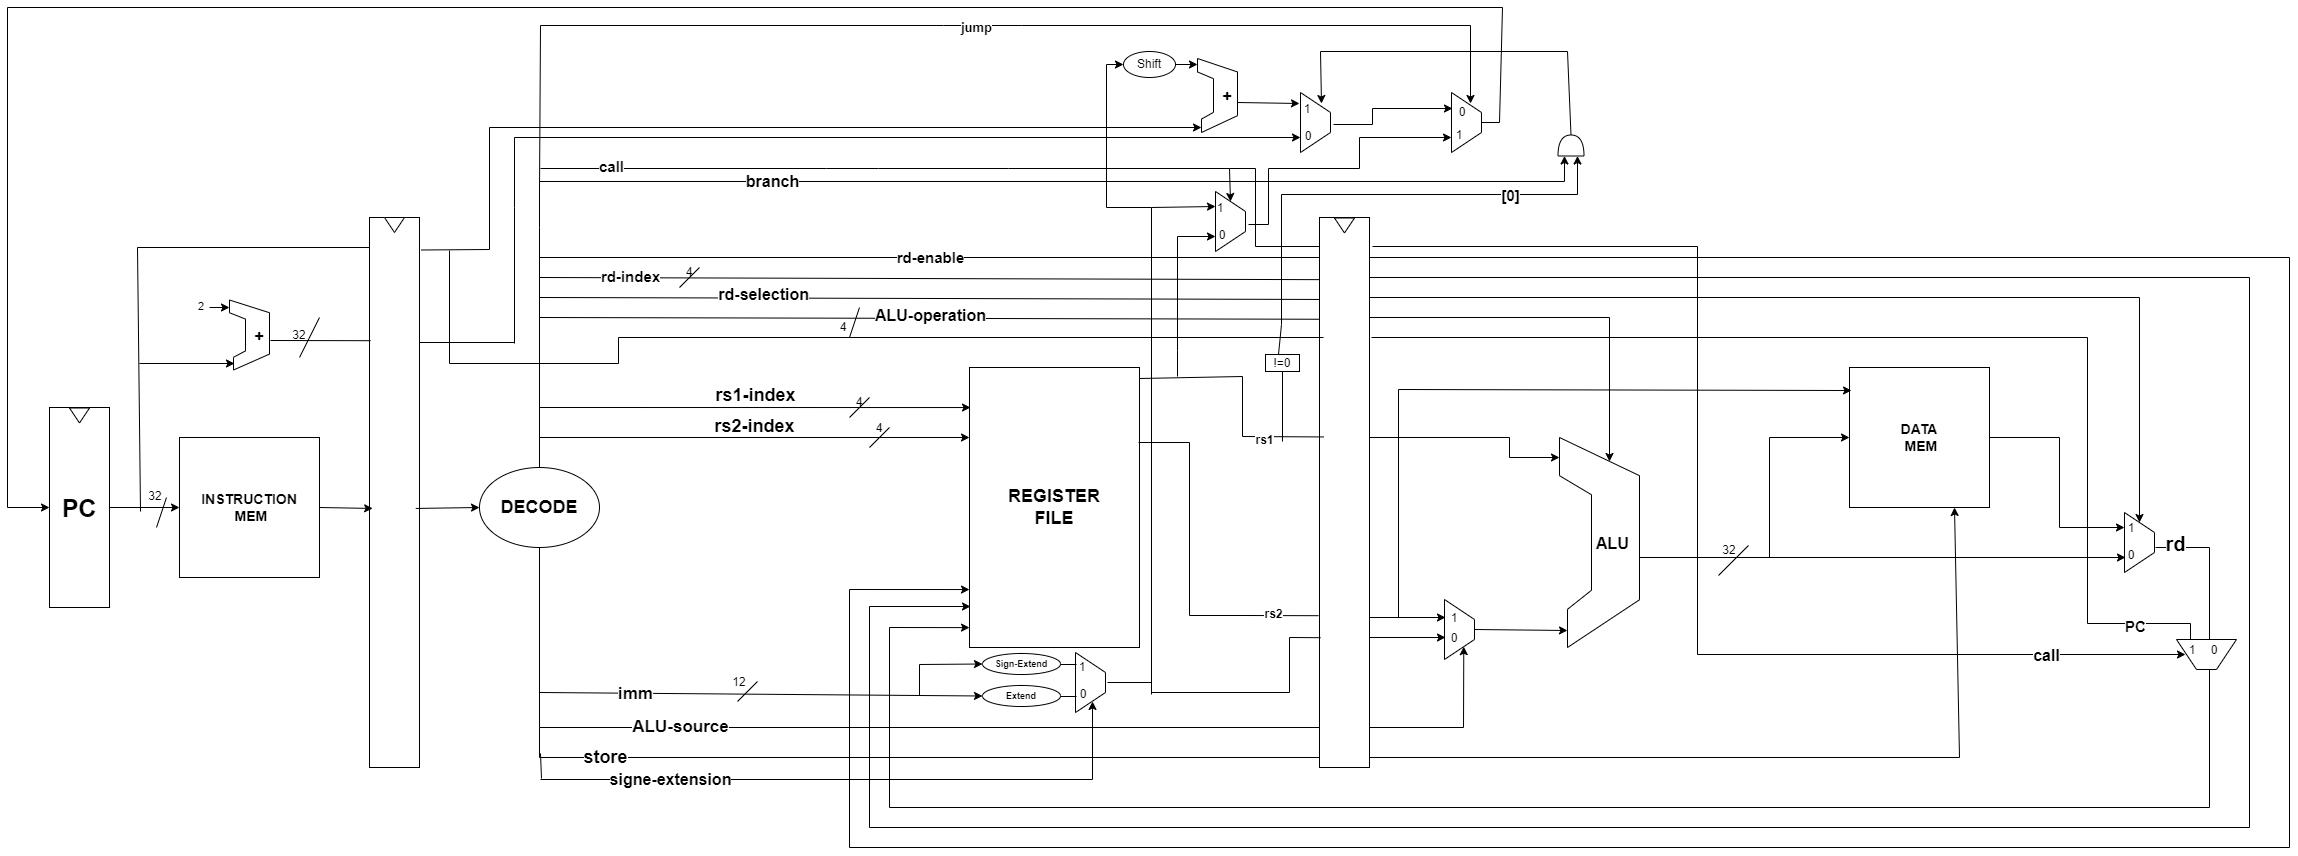
\includegraphics[width=1\linewidth]{RISCV.png}
    \caption{Processor scheme}
    \label{fig:processor-scheme}
\end{figure}

\textbf{Processor characteristics :}

\begin{itemize}
    \item It has three pipeline stages, IF, ID, and EX, and makes use of three memories; Instruction Memory, Register Files and Data Memory.
    \item For arithmetic operations, the pipeline stages correspond as the result is computed and stored in the register file during the EX stage.
    \item For memory access, the address computation and the memory access are both done during the EX stage.
    \item Branches, jumps, and calls are executed during the ID stage.
    \item The registers are written at the beginning of the EX stage and read at the end of the ID stage.
\end{itemize}

\textbf{Program counter specifications :} \\

The Program Counter (PC) block is implemented as a synchronous register to ensure the stability of the instruction memory during the Instruction Decode (ID) stage and to effectively separate the Instruction Fetch (IF) and ID stages.\\

To maintain efficient operation and avoid delays in incrementing the PC value, the initialization process must be carefully managed. Specifically, the PC register should be initialized to 0 at processor start-up. Simultaneously, the IF/ID pipeline register holding the PC + 2 value should be set to 2. This initialization ensures that the PC increment operation does not require two clock cycles to complete, thereby optimizing the instruction fetch process.\\

\textbf{The functioning of the processor : }\\

The decoder extracts various elements from the binary form of the instruction, preparing them for use by different components of the processor :

\begin{itemize}
    \item \textbf{jump} : Set to 1 if the instruction is a jalr or call instruction; otherwise, set to 0.
    \item \textbf{call} : Set to 1 if the instruction is a call instruction; otherwise, set to 0.
    \item \textbf{branch} : Set to 1 if the instruction is a bne instruction; otherwise, set to 0.
    \item \textbf{rd-index, rs1-index and rs2-index} : Indicate the indices of the destination (rd) and the source registers (rs1 and rs2) within the instruction. These indices are used to read from or write to the register file.
    \item \textbf{ALU-operation} : Allows to select the operation done by the Arithmetic Logic Unit (ALU).
    \item The decoder also extracts a 12-bit immediate value from the instruction, and a sign-extension bit is generated to enable or disable the sign extension of this immediate value, depending on the type of instruction.
\end{itemize}

To handle arithmetic operations, our processor employs an Arithmetic Logic Unit (ALU). This ALU performs arithmetic operations between registers or between a register and an immediate value.\\

Multiplexers are used to manage the inputs for these operations. The decoder generates control signals for these multiplexers, such as:

\begin{itemize}
    \item \textbf{sign-extension} : Determines whether the immediate value should be sign-extended or not.
    \item \textbf{ALU-source} : Controls whether the second operand for the ALU is an immediate value or the content of the register indexed by the rs2-index.
    \item \textbf{rd-selection} : Allows the selection of the signal directed to the rd register, choosing between the outputs of the Arithmetic Logic Unit (ALU) and the data memory.
\end{itemize}

Multiplexers also control the PC value before each instruction execution. The selection of the next PC value is influenced by the CALL, BRANCH, and JUMP signals generated by the decoder.\\

Furthermore, the decoder generates control bits to manage memory operations:
\begin{itemize}
    \item \textbf{rd-enable} : When set to 1, it enables writing the result at the end of the execution stage (EX) to the register file.
    \item \textbf{store} : When set to 1, it allows data to be written to the data memory.
\end{itemize}

\textbf{Call instruction execution :}\\

We illustrate the execution of the call instruction inside the processor.

\begin{figure}[H]
    \centering
    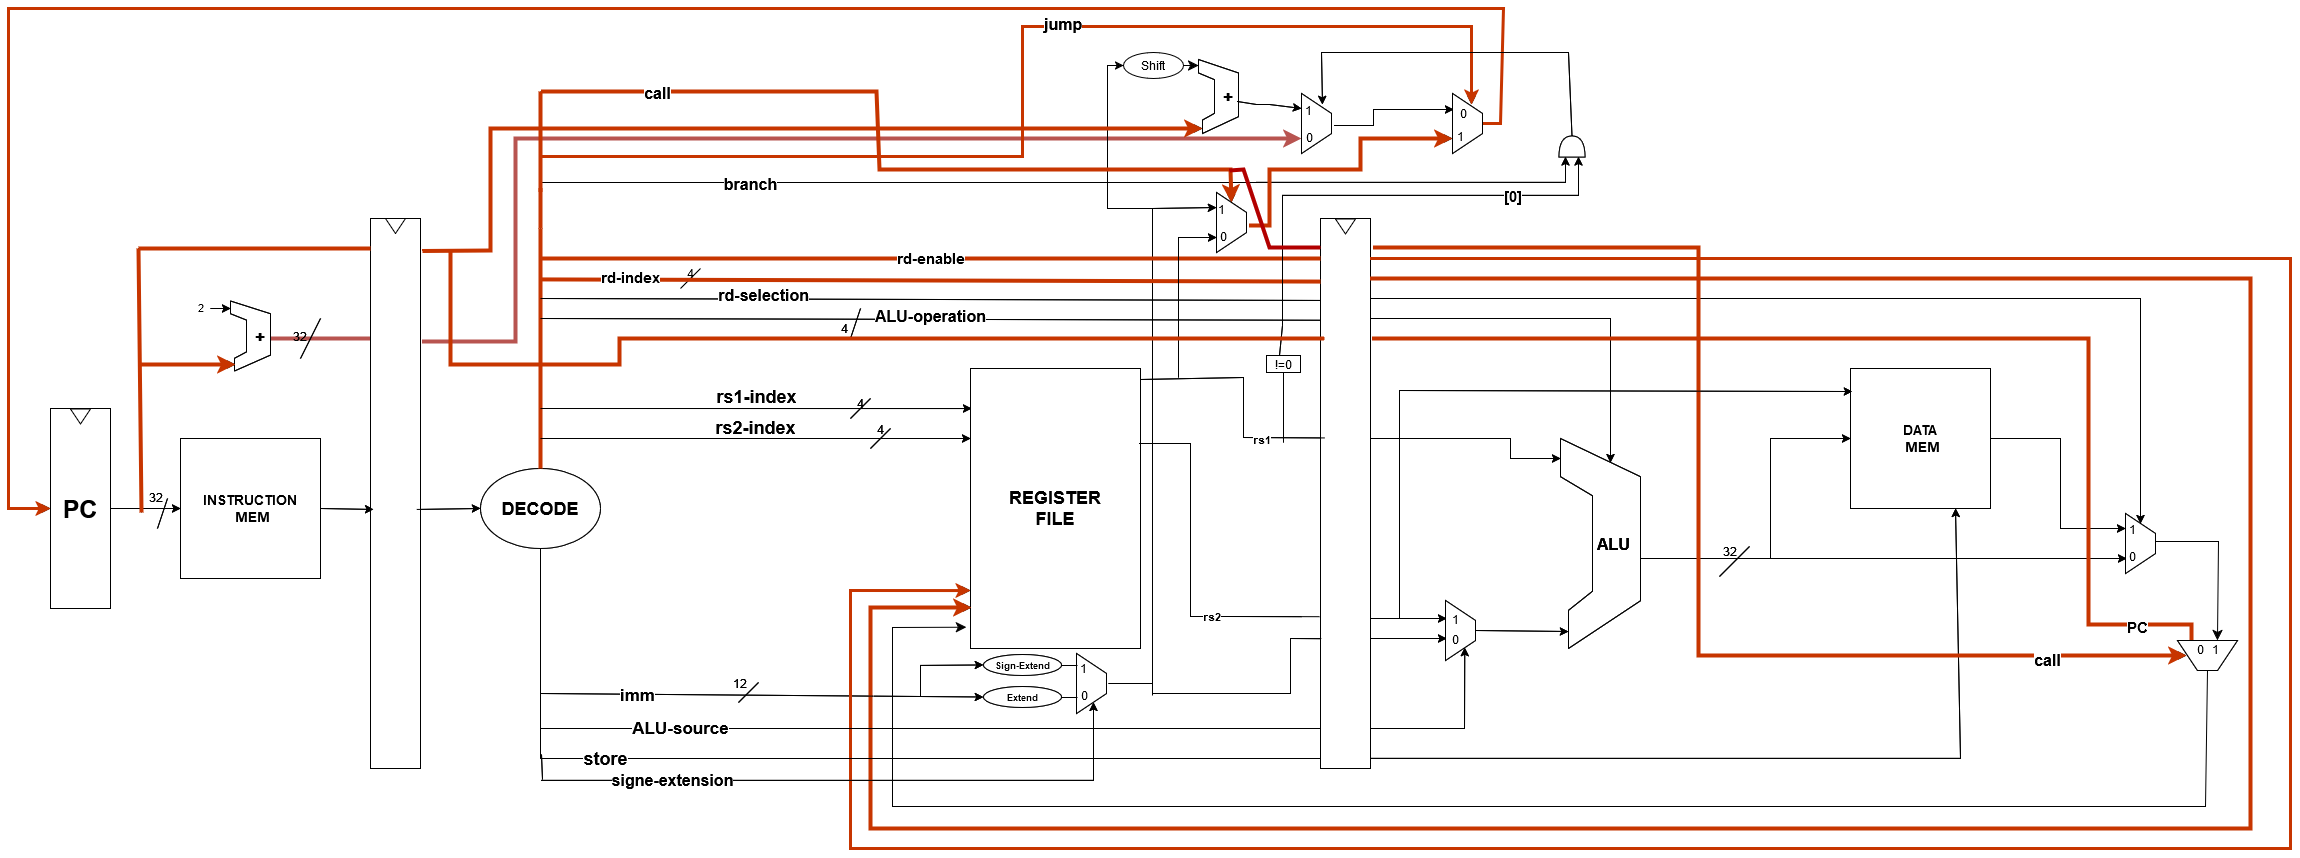
\includegraphics[width=1\linewidth]{CALL_instruction.png}
    \caption{Call instruction execution}
    \label{fig:call-exe}
\end{figure}

The visual representation of the system includes highlighted wires to indicate significant data paths. A highlighted wire signifies either a value of 1, if it represents a single bit, or an important instruction-related value, if it represents multiple bits.\\

\textbf{Explanation :} \\

Upon encountering a "Call" instruction in the instruction memory. The binary format of the instruction is passed through the IF/ID register pipeline and sent to the decoder, which generates the necessary control signals to manage multiplexers, registers, and other components.\\

When the instruction reaches the IF/ID register pipeline, the ID stage begins. The decoder identifies the binary format as a "Call" instruction and generates the following control signals:
\begin{itemize}
    \item \textbf{call bit} : Set to 1 to indicate a Call instruction.
    \item \textbf{jump bit} : To indicate a jump instruction independent of PC
    \item \textbf{Immediate value} : A 12-bit immediate value extracted from the instruction.
    \item \textbf{sign-extension bit} : Set to 0, as the immediate in call instructions is not sign-extended.
\end{itemize}

Since the call instruction modifies the content of the r1 register, the decoder generates a 4-bit index (0001) for r1 as input to the register file. Additionally, the rd-enable bit is set to 1 to allow writing to the register file during the EX stage of the pipeline.\\

It is important to note that the ID stage computes the PC value of the next instruction. However, it will take an additional clock cycle for it to be available in the IF stage. This delay is a consequence of the pipeline structure, as demonstrated in the table below.\\

This diagram illustrates what is happening from the pipeline point of view :
\begin{table}[H]
\centering\begin{tabular}{|l|lllll|}
\hline
\textbf{Instructions}                                                       & \multicolumn{5}{l|}{\textbf{Cycles}}                                                                                                                                                          \\ \hline
PC : call \#new\_PC                                                         & \multicolumn{1}{l|}{IF} & \multicolumn{1}{l|}{ID}                                                                                    & \multicolumn{1}{l|}{EX} & \multicolumn{1}{l|}{}   &    \\ \hline
\begin{tabular}[c]{@{}l@{}}PC + 2 : instruction\\ (delay slot)\end{tabular} & \multicolumn{1}{l|}{}   & \multicolumn{1}{l|}{IF}                                                                                    & \multicolumn{1}{l|}{ID} & \multicolumn{1}{l|}{EX} &    \\ \hline
new\_PC : instruction                                                       & \multicolumn{1}{l|}{}   & \multicolumn{1}{l|}{\begin{tabular}[c]{@{}l@{}}PC became new\_PC at \\ the end of this cycle\end{tabular}} & \multicolumn{1}{l|}{IF} & \multicolumn{1}{l|}{ID} & EX \\ \hline
\end{tabular}
    \caption{Pipeline diagram of a call instruction}
    \label{tab:pipeline-diagram-2}
\end{table}
In the Execute (EX) stage, when a call instruction is executed, the address of the instruction represented by the current Program Counter (PC) value is captured and stored in the r1 register. This process is managed by setting the rd-enable bit to 1, which initiates an update of the register file, and setting the call signal to 1. The call signal directs the rd register to be linked with the PC value, rather than the Arithmetic and Logic Unit (ALU) or data memory outputs. Consequently, the r1 register is updated to hold the address of the Call instruction, ensuring that return addresses are effectively handled during procedure calls.\\

\textbf{Hazards :}

\begin{itemize}
    \item \textbf{Data Hazards : }Due to the last characteristic of our processor, which states that registers are written at the beginning of EX state, and read at the end of the ID stage. We deduced that data hazards will never occur, because the registers can never be read before being written. Accordingly, we will not need to implement forwarding or stalling in our processor.
    \item \textbf{Control Hazards : }This type of hazard can occur in the processor due to the our pipeline structure: where the decision to perform a jump is made, while in the IF stage, the next instruction is already being fetched. To address this hazard, a branch delay slot is introduced after each \texttt{call}, \texttt{jal}, or \texttt{bne} instruction. By ensuring that the branch delay slot is always respected, the need for flushing can be avoided.
    \item \textbf{Structural Hazards :}This kind of hazards does not affect our processor mainly due to its last characteristic, mentioned above.
\end{itemize}

\textbf{Flushing :}\\

If branch delay slots are properly respected during the writing or generation of the assembly code, flushing will not be necessary. However, in cases where flushing is required, it can be implemented by first detecting the need for it. This detection can be achieved by applying an OR gate to the signals indicating a jump occurrence. Once detected, the result can be routed through a multiplexer, which will send the NOP instruction to the IF/ID register. As a result, the NOP instruction will be executed in the ID and EX stages, allowing for an efficient flush with minimal logic.

\end{document}